\documentclass[11pt]{article}

\usepackage{courier}            % standard fixed width font
\usepackage[scaled]{helvet} % see www.ctan.org/get/macros/latex/required/psnfss/psnfss2e.pdf
\usepackage{url}                  % format URLs
\usepackage{listings}          % format code
\usepackage{enumitem}      % adjust spacing in enums
\usepackage[tight,hang]{subfigure}
\usepackage{xspace}
\usepackage{graphicx}
\usepackage{mathtools}
\usepackage{mathpartir}
%\usepackage{minionpro}
\usepackage{amssymb}
\usepackage{amsmath}
\usepackage{amsfonts}
\usepackage{fullpage}
\usepackage{ifpdf}
\usepackage{deauthor, times}
\usepackage[usenames,dvipsnames]{color}
\usepackage{stmaryrd}
\usepackage[numbers]{natbib}
\usepackage{wrapfig}
\usepackage{textcomp}

\ifpdf
  \usepackage{hyperref}
  \usepackage{graphicx}
\else
  \usepackage[dvips]{graphicx}
  \usepackage[dvips]{hyperref}
\fi

\newcounter{copyrightbox}

% Listings
%----------
\lstloadlanguages{haskell}
\newcommand{\lsthaskell}{\lstset{
      language=haskell,
      %basicstyle=\ttfamily\ninett\footnotesize,
      flexiblecolumns=false,
			tabsize=2,
      %basewidth={0.5em,0.45em},
      %aboveskip={3pt},
      %belowskip={3pt},
      keywordstyle=\color{blue}\bfseries,
      commentstyle=\color{darkgreen}\itshape,
      morekeywords={foldl,fold},
			classoffset=1,
			upquote=true,
			keywordstyle=\color{Fuchsia}\bfseries,
			classoffset=0,
			mathescape=true,
      literate={+}{{$+$}}1 {/}{{$/$}}1 {*}{{$*$}}1 % {=}{{$=$}}1
               {>}{{$>$}}1 {<}{{$<$}}1
							 {dollar}{{\$}}1
               {\\\\}{{\char`\\\char`\\}}1
               {->}{{$\rightarrow$}}2 {>=}{{$\geq$}}2 {<-}{{$\leftarrow$}}2
               {<=}{{$\leq$}}2 {=>}{{$\Rightarrow$}}2
               {\ .}{{$\circ$}}2 {\ .\ }{{$\circ$}}2
               {>>}{{>>}}2 {>>=}{{>>=}}2 {=<<}{{=<<}}2
               {|}{{$\mid$}}1
							 {(-}{{$\in$}}1
						   {psi1}{{$\psi_1$}}1 {psi2}{{$\psi_2$}}1
							 {cup}{{$\cup$}}1
							 {cap}{{$\cap$}}1
							 {forall}{{$\forall$}}1
							 {vee}{{$\vee$}}1
							 {wedge}{{$\wedge$}}1
               {`member`}{{$\in$}}1
               {s.empty}{{\{\}}}1
               {leftbrace}{\{}1
               {rightbrace}{\}}1
               {profile0sing}{{ \{{\tt profile0}\}}}1
               {\$singleton\$startv}{{ \hspace{2.4em} \{{\tt startv}\}}}1
               {\$singleton\$n}{{  \{{\tt n}\}}}1
               {dotdotdot}{{$\ldots$}}3
    }}
\lstnewenvironment{codehaskell}
    { % \centering
			\lsthaskell
      \lstset{}%
      \csname lst@setfirstlabel\endcsname}
    { %\centering
      \csname lst@savefirstlabel\endcsname}

% Formatting
%---------
\newcommand{\scc}{\psi_{\sf sc}}
\newcommand{\ccc}{\psi_{\sf cc}}
\newcommand{\ecc}{\psi_{\sf ec}}
\newcommand{\rcc}{\psi_{\sf rc}}
\newcommand{\mavc}{\psi_{\sf mav}}
\newcommand{\rrc}{\psi_{\sf rr}}
\newcommand{\coloneqq}{::=}

% \newtheorem{theorem}{Theorem}
% \newtheorem{lemma}[theorem]{Lemma}
% \newtheorem{proposition}[theorem]{Proposition}
% \newtheorem{corollary}[theorem]{Corollary}
% \newtheorem{definition}[theorem]{Definition}
\newcounter{hno}
\newcounter{gno}
\renewenvironment{proof}{\setcounter{hno}{0}\setcounter{gno}{0}
  \emph{Proof.}}{}
\newcommand{\npp}{\thehno \stepcounter{hno}}
\newcommand{\mpp}{\thegno \stepcounter{gno}}

\newcommand{\stretcharraybig}{\renewcommand*{\arraystretch}{1.25}}
\newcommand{\cureff}{\hat{\eta}}
\newcommand{\eff}{\eta}
\newcommand{\fresh}{\N{\sf fresh}}
\newcommand{\cv}{\psi}
\newcommand{\ALT}{~\mid~}
\newcommand{\eid}{{\iota}}
\newcommand{\ObjType}{{\sf ObjType}}
\newcommand{\AbsType}{{\sf AbsType}}
\newcommand{\dom}{{\sf dom}}
\newcommand{\DtLib}[1]{\mathbb{D}(#1)}
\newcommand{\DtLibZ}{\mathbb{D}}
\newcommand{\Ops}{\Lambda}
\newcommand{\Ctrts}{\Psi}
\newcommand{\true}{\N{\textsf{true}}}

\newcommand{\R}[1]{\textrm{#1}}
\newcommand{\N}[1]{{\normalfont #1}}
\newcommand{\ObjZ}{\N{\textsf{Obj}}}
\newcommand{\Obj}[1]{\N{\textsf{Obj}_{#1}}}
\newcommand{\ReplID}{\mathtt{ReplID}}
\newcommand{\SessID}{\mathtt{SessID}}
\newcommand{\typeFun}[1]{\N{\textsf{type}}(#1)}
\newcommand{\Op}[1]{\N{\textsf{Op}_{#1}}}
\newcommand{\set}[1]{\overline{#1}}
\newcommand{\unitVal}{\N{\textsf{unit}}}
\newcommand{\EffUniv}{\N{\sf Effect}}
\newcommand{\EffID}{\mathtt{SeqNo}}
\newcommand{\TransID}{\N{\sf TransID}}
\newcommand{\AVal}[1]{\N{\textsf{AVal}_{#1}}}
\newcommand{\RVal}[1]{\N{\textsf{RVal}_{#1}}}
\newcommand{\Eff}[1]{\N{\textsf{Eff}_{#1}}}
\newcommand{\loud}[1]{\textbf{\textit{#1}}}
\newcommand{\dt}[1]{\mathcal{D}_{#1}}
\newcommand{\vis}[2]{\N{\textsf{vis}(#1,#2)}}
\newcommand{\visZ}{\N{\textsf{vis}}}
\newcommand{\depsZ}{\N{\textsf{deps}}}
\newcommand{\deps}[1]{\N{\textsf{deps}(#1)}}
\newcommand{\Rvis}{\N{\textsf{vis}}}
\newcommand{\arZ}{\N{\textsf{ar}}}
\newcommand{\ar}[2]{\N{\textsf{ar}(#1,#2)}}
\newcommand{\stxZ}{\sim}
\newcommand{\stx}[2]{#1\sim#2}
\newcommand{\nstx}[2]{#1\not\sim#2}
\newcommand{\comZ}{\N{\textsf{com}}}
\newcommand{\com}[1]{\comZ(#1)}
\newcommand{\so}[2]{\N{\textsf{so}(#1,#2)}}
\newcommand{\soZ}{\N{\textsf{so}}}
\newcommand{\stZ}{\N{\textsf{st}}}
\newcommand{\Rso}{\N{\textsf{so}}}
\newcommand{\Rst}{\N{\textsf{st}}}
\newcommand{\COM}{\textrm{\sc {\small Commit}}}
\newcommand{\soo}[2]{\N{\textsf{soo}(#1,#2)}}
\newcommand{\sooZ}{\N{\textsf{soo}}}
\newcommand{\hb}[2]{\N{\textsf{hb}(#1,#2)}}
\newcommand{\hbo}[2]{\N{\textsf{hbo}(#1,#2)}}
\newcommand{\hbZ}{\N{\textsf{hb}}}
\newcommand{\hboZ}{\N{\textsf{hbo}}}
\newcommand{\oper}[2]{\N{\textsf{oper}(#1,#2)}}
\newcommand{\operZ}{\N{\textsf{oper}}}
\newcommand{\txnZ}{\N{\textsf{txn}}}
\newcommand{\txn}[2]{\txnZ\{#1\}\{#2\}}
\newcommand{\sameobj}[2]{\N{\textsf{sameobj}(#1,#2)}}
\newcommand{\sameobjZ}{\N{\textsf{sameobj}}}
\newcommand{\sametxn}[2]{\N{\textsf{sametxn}(#1,#2)}}
\newcommand{\sametxnZ}{\N{\textsf{sametxn}}}
\newcommand{\E}{\N{\textsf{E}}}
\newcommand{\EffSoup}{\N{\textsf{A}}}
\newcommand{\obj}{\N{\textsf{obj}}}
\newcommand{\dep}{\N{\textsf{dep}}}
\newcommand{\rval}{\N{\textsf{rval}}}
\newcommand{\repl}{\N{\textsf{repl}}}
\newcommand{\sess}{\N{\textsf{sess}}}
\newcommand{\rdtspec}{\Delta}
\newcommand{\goesto}{\longrightarrow}
\newcommand{\tuplee}[1]{\langle #1 \rangle}
\newcommand{\ctxtFn}{\N{\textsf{ctxt}}}
\newcommand{\rdtredsto}{\N{\leadsto}}
\newcommand{\Exec}{\N{\textsf{(\EffSoup,\allowbreak \visZ,\allowbreak \soZ,\allowbreak \sameobjZ)}}}
\newcommand{\pll}{~\|~}
\newcommand{\Mod}[1]{\N{\textsf{Mod}}(#1)}
\newcommand{\De}[1]{[\![#1]\!]}
\newcommand{\Der}[2]{[\![#1,#2]\!]_{r}}
\newcommand{\msentails}[2]{#1 \models #2}
\newcommand{\hasTyp}[2]{#1 \vdash #2}
\newcommand{\auxred}[4]{#1 #2 \;\xrightarrow{#3}\; #4 }


% Operational semantics rules
\newcommand{\rulelabel}[1]{\textrm{\sc {\small [#1]}}}
\newcommand{\RULE}[3]
{\frac{\begin{array}{c}#1\end{array}}
		 {\begin{array}{c}#2\end{array}}
~ \rulelabel{#3}
}

\newcommand{\RuleTwo}[2]
{\frac{\begin{array}{c}#1\end{array}}
		 {\begin{array}{c}#2\end{array}}
}

\newenvironment{nop}{}{}
\newenvironment{smathpar}{
\begin{nop}\small\begin{mathpar}}{
\end{mathpar}\end{nop}\ignorespacesafterend}

\newenvironment{cmathpar}{
\vspace{-3mm}
\renewcommand{\arraystretch}{1.2}
\begin{nop}\begin{mathpar}}{
\end{mathpar}\end{nop}\ignorespacesafterend}

\newcommand{\rsf}[1]{\R{\sf #1}}
\newcommand{\trans}[4]{\N{\textsf{trans}}\{#1,#2\}\{#3,#4\}}

\newcommand{\name}{{\sc Quelea}\xspace}
\newcommand{\ecds}{ECDS\xspace}


%% KC spacing edits -- should be removed eventually -- Fix the text!
\setlength{\floatsep}{5pt}
\setlength{\textfloatsep}{10pt}
\setlength{\dblfloatsep}{5pt}
\setlength{\dbltextfloatsep}{10pt}

\newcommand{\C}[1]{\code{#1}}
\newcommand{\inang}[1]{\langle #1 \rangle}

% Formatting commands
% -------------------
\newcommand{\code}[1]{\,{\tt #1}\,}
\newcommand{\cf}[1]{{\small\tt #1}}
\newcommand{\rcf}[1]{\ensuremath{\mathrm{\cf{#1}}}}
\newcommand{\spc}[0]{\quad}
\newcommand{\rel}[1]{{R}_{\mathit{#1}}}
\newcommand{\conj}{~\wedge~}
\newcommand{\disj}{~\vee~}
\newcommand{\ilrulelabel}[1]{{\sc #1}}
\date{}
\begin{document}

\title{A Language Framework for Programming With Weak Consistency and
Isolation}
%\subtitle{Research Summary}

% \author{Gowtham Kaki \\ \small{Purdue University} \hspace*{0.1in}
%   \small{{\tt gkaki@purdue.edu}} }

\maketitle

\begin{abstract}
% Due to the inevitable tradeoff between consistency and availability in
% an asynchronous distributed system, a geo-distributed application is
% forced to choose between either being strongly consistent or being
% highly availabile. Motivated by the strong correlation between high
% availability and user satisfaction, 
Geo-distributed web applications often favor high availability over
strong consistency. Reacting to their needs, modern-day replicated
data stores eschew sequential consistency in favor of weaker eventual
consistency (EC). While most operations a typical web application
supports can be engineered to function under EC, there nonetheless
exist a few critical operations that require stronger consistency
guarantees. Few off-the-shelf eventually consistent key-value stores
do offer tunable consistency levels to address the need. However,
these consistency levels often have poorly-defined ad hoc semantics
that is too low-level from the perspective of an application, and
often strongly tied to the respective implementations of the data
store. While such low-level implementation-dependent solutions do not
readily cater to the high-level requirements of an application,
relying on ill-defined guarantees may even complicate the already-hard
task of reasoning about application semantics under eventual
consistency. 

In this paper, we describe \name, a declarative programming model for
eventually consistent data stores. A novel aspect of \name is that it
completely abstracts the actual implementation of the data store, thus
delivering application programmers from having to reason about their
application in terms of the low-level implementation-specific
semantics of the data store. Instead, programmers can reason in terms
of an abstract model of the data store, and develop applications by
defining and composing high-level replicated data types. \name is
equipped with a formal specification language that is capable of
expressing precise semantics of high-level consistency guarantees
(eg., causal consistency) in the abstract model. Any eventually
consistent key-value store can support \name by implementing a thin
shim layer and a choosen set of high-level consistency guarantees on
top of its existing low-level interface. We describe one such
implementation of \name on top of Cassandra, complete with the support
for causal and sequential consistency guarantees, and
coordination-free transactions. We present a case study of a large web
application benchmark demonstrate the practical utility of \name.


\end{abstract}

\section{Introduction}
\label{sec:intro}

Eventual consistency facilitates high availability, but can lead to
surprising anomalies that have been
well-documented~\cite{Burckhardt2014, pldi15, Session, Dynamo,
  RedBlue}. While applications can often tolerate many of these
anomalies, there are some that adversely effect the user experience,
and hence need to be avoided. For instance, a social network
application can tolerate out-of-order delivery of unrelated posts, but
causally related posts need to be delivered in causal order;
\emph{e.g.,}, a comment cannot be delivered before the post
itself. The view count of a video on Youtube need not necessarily
reflect the precise count of the number of views, but it should not
appear to be decreasing. A bank account application may not always
show the accurate balance in an account, but neither should it let the
balance go below zero, nor should it admit operations that would
lead it to display a negative balance.

Bare eventual consistency is often too weak to ensure such high-level
application invariants; stronger consistency guarantees are needed. To
help applications enforce such high-level invariants, off-the-shelf
replicated data stores, such as Cassandra and Riak, offer tunable
consistency levels on a per-operation basis: applications can specify
the consistency level for every read and write operation they perform
on the data store. However, consistency levels offered by these
off-the-shelf stores are often defined at a very low-level. For
example, consistency levels in Cassandra and Riak assume the values of
\C{ONE}, \C{TWO}, \C{QUORUM}, \C{ALL} etc., desribing how many
physically distributed comprising the store must respond before a read
or write operation is declared successful.  It is not immediately
apparent what permutation of these low-level consistency guarantees
would let the application enforce its high-level level invariants. For
instance, what should be the consistency level of reads and writes to
the \C{posts} table\footnote{We use the word \emph{table} as an
  all-encompassing term for various key-value abstractions provided by
  data stores.} to guarantee causal order delivery of posts in the
aforementioned social network application?

Furthermore, the semantics of low-level consistency guarantees are not
uniform across different store implementations. For instance, while
\C{QUORUM} means \emph{strict quorum} (i.e., Lamport's
quorum~\cite{LamportQuorum}) in the case of Cassandra, it means a
\emph{sloppy quorum}~\cite{Dynamo} in Riak. Complicating matters yet
further, consistency semantics is often imprecisely, or even
inaccurately, defined in the informal vendor-hosted documentations.
For instance, Datastax's Cassandra documentation~\cite{dxlwt} claims
that one can achieve ``strong consistency'' with ``quorum reads and
writes'' in Cassandra.  While this claim appears reasonable
superficially (because a pair of quorum operations are serialized at
one node, at least), it is incomplete, at best, and inaccurate at
worst.\footnote{The devil is in the details of the timestamp-based
  last-writer-wins conflict resolution strategy in Cassandra, which
  need not necessarily pick the last writer due to inevitable clock
  drift across nodes.~\cite{TyconCassandra} and~\cite{JepsenCassandra}
  present counterexamples and a more accurate claim.}  Another example
of a low-level consistency enforcement construct with vaguely defined
semantics is Cassandra's Compare-and-Set ({\sc cas}) operation, which
is advertised as a ``lightweight transaction'' and exposed as a
conditional write query (eg., \C{INSERT INTO users VALUES … IF NOT
  EXISTS}).  The addition of {\sc cas} to Cassandra was coupled with
the introduction of a new consistency level named \C{SERIAL}.
Surprisingly, \C{SERIAL} is not a valid query-level consistency
parameter for a write (conditional or not), while the others
(\emph{e.g.}, \C{ONE}) are valid.\footnote{Given the advertised use
  cases for lightweight transactions (such as maintaining uniqueness
  of usernames), one might expect a {\sc cas} to be \C{SERIAL} by
  default. It is therefore unintuitive that {\sc cas} accepts a
  consistency parameter, at least to the developers of cassandra-cql,
  a popular Haskell library for programming with Cassandra, whose API
  for {\sc cas} operation incorrectly hardcodes the parameter to
  \C{SERIAL}. This bug has been reported and fixed.}  Furthermore,
Cassandra accepts a new \emph{protocol-level} consistency parameter
for a {\sc CAS} operation that can be set to \C{SERIAL}, but its
informal description doesn't explain how this parameter interacts with
the query-level consistency parameter.  The only way to unravel this
complexity is to understand low-level details of the operator's
underlying Paxos-based implementation.  Mired in this quagmire of
low-level implementation details, it is easy to lose track of our
original goal - ensuring the high-level semantics guarantees required
by the application are met as efficiently as possible by the
implementation.

In this paper, we describe \name, a declarative programming framework
for eventually consistent data stores that was build to address the
issues discussed above. \name can be realized as a thin layer on top
of any off-the-shelf eventually consistent key-value store, and as
such, provides a uniform implementation-independent interface to the
data store. \name programmers reason in terms of an abstract system
model of an eventually consistent data store (ECDS), and any
functionality offered by the store in addition to bare eventual
consistency, including stronger consistency guarantees, transactions
with tunable isolation levels etc., is required to have a well-defined
semantics in the context of this abstract model. We show that various
high-level consistency guarantees (eg., causal consistency) and
various well-known isolation levels for transactions (eg., read
committed) indeed enjoy such properties.  \name is additionally
equipped with an expressive specification language that lets data
store developers succintly describe the semantics of the functionality
they offer. A similar specification language is exposed to application
programmers, who can declare the consistency requirements of their
application as axiomatic specifications. Specifications are
constructed using primitive consistency relations such as
\emph{visibility} and \emph{session order} along with standard logical
and relational operators. A novel aspect of \name is that it can
directly compare the specifications written by application programmers
and data store developers since both are written within the same
specification language, and can thus automatically map application
requirements to the appropriate store-level guarantees. Consequently,
\name programmers can write portable code that automatically adapts to
any data store that can express its functionality in terms of \name's
abstract system model.

Another key advantage of \name is that it allows the addition of new
replicated data types (RDTs) to the store, which obviates the need to
support data types with application-specific semantics at the store
level. In addition, \name treats the convergence semantics (i.e.,
\emph{how} conflicting updates are resolved) of the data type
separately from its consistency properties (i.e., \emph{when} updates
become visible).  This separation of concerns permits
\emph{operational} reasoning for conflict resolution, and
\emph{declarative} reasoning for consistency.  The combination of
these techniques enhances overall programmability and simplifies
reasoning about application correctness.

% Rest of this paper is organized as following. The next section
% describes the abstract system model. The following section describes a
% sample application to demonstrate the style of programming promoted by
% \name. We also cover the anomalies exhibited by the application under
% eventual consistency, which highlights the need for stronger
% consistency guarantees with well-defined high-level semantics.
% ~\S~\ref{sec:language} introduces \name's specification language, and
% presents the specifications of various high-level consistency
% guarantees. 


\section{System Model}
\label{sec:sysmod}

\begin{figure}
\centering
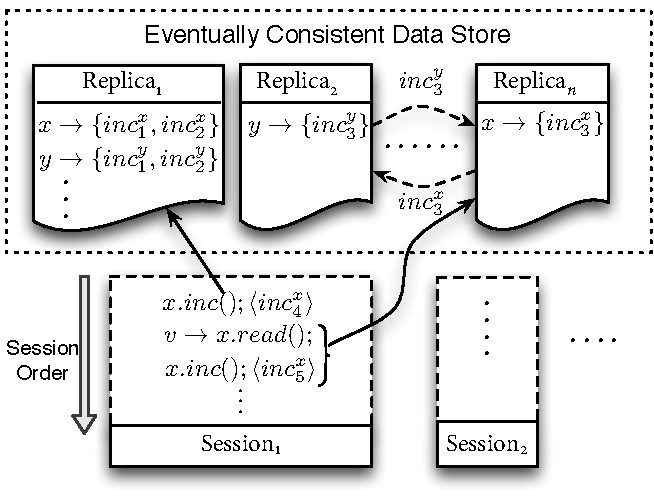
\includegraphics[scale=0.9]{Figures/SystemModel}
\caption{\name system model.}
\label{fig:sysmod}
\end{figure}

Figure~\ref{fig:sysmod} summarizes the abstract system model of a data
store exposed to the \name programmer. The store is a collection of
\emph{replicas}, each storing a set of \emph{objects} ($x,y,\ldots$)
of a replicated data type. For the sake of an example,  let $x$ and
$y$ represent objects of an \emph{increment-only counter} replicated
data type (RDT) that admits \emph{inc} and \emph{read} operations. The
state of an RDT object is represented as the set of all updates
(effectful operations, or simply \emph{effects}) performed on the
object. In Fig.~\ref{fig:sysmod}, the state of $x$ at replica 1 is the
set $\{inc^x_1,inc^x_2\}$, where each $inc^x_i$ denotes an \emph{inc}
effect on $x$.

Clients interact with the data store via concurrent \emph{sessions},
where each session is a sequence of operations that a client invokes
on any of the objects contained in the store. Note that clients have
no control over which replica an operation is applied to; the data
store may choose to route the operation to any replica in order to
minimize latency, load balance, etc. For example, the \emph{inc} and
\emph{read} operations invoked by the same session on the same object,
may be applied on different replicas because replica 1 (to which the
\emph{inc} operation is applied, say) might be unreachable when the
client invokes a subsequent \emph{read}.

When an operation is applied to a replica, it is said to witness the
state of its object at that replica.  For example, \emph{x.inc}
applied to replica 1 witnesses the state of $x$ as
$\{inc^x_1,inc^x_2\}$.  We say that the effects $inc^x_1$ and
$inc^x_2$ are \emph{visible} to the effect ($inc^x_4$) of
\emph{x.inc}, written logically as $\small \vis{inc^x_1}{inc^x_4}
\wedge \vis{inc^x_2}{inc^x_4}$, where $\small \visZ$ stands for the
irreflexive and asymmetric visibility relation between effects over
the same object. The notion of visibility is important since the
result of an operation often depends on the set of visible
effects\footnote{We abuse the visibility relation by informally
  extending it to operations (including read-only operations, which
  produce no effects).}. For instance, a \emph{read} on $x$ applied to
the last replica in Fig.~\ref{fig:sysmod} returns 1 since it only
witnesses the effect ($inc^x_3$) of a single \emph{x.inc} operation.

A visibility relation between two effects implies that the former
operation has happened before the latter (since the latter has
witnessed the effect of the former). However, visibility is not enough
to capture a happens-before order between operations. As
Fig.~\ref{fig:sysmod} demonstrates, a pair of operations from the same
session, although one happens before the other, need not be visible to
each other. To capture happens-before, we define an irreflexive
transitive \emph{session order} relation that relates the effects of
operations arising from the same session. For example, in
Fig.~\ref{fig:sysmod}, $inc^x_4$ and $inc^x_5$ are in session order
(written logically as $\small \so{inc^x_4}{inc^x_5}$).

The effect added to a particular replica is asynchronously sent to
other replicas, and eventually merged into all other replicas. Observe
that this model is independent of the resolution strategy for
concurrent conflicting updates, and instead preserves \emph{every}
update. Update conflicts are resolved when an operation reduces over
the set of effects on an object at a particular replica. The model,
however, admits all the inconsistencies associated with eventual
consistency, some of which could adversely impact the usability of the
application. We call such unacceptable inconsistencies as
\emph{anomalies}. Stronger consistency guarantees are needed to
prevent unwanted anomalies.

In the next section we concretize, in \name, the \emph{counter}
application described informally above, followed by the anomalies the
application admits under our model.  Next, we show that strengthening
the model with a few simple guarantees is enough to prevent these
anomalies. We introduce a specification language that lets us
naturally express such additional requirements. Finally, we show that
well-known high-level consistency guarantees have precise semantics
under our model, and hence can be expressed as formulas in our
specification language. This makes it straightforward to compare
application requirements with consistency guarantees, and determine
the appropriate consistency semantics required to prevent anomalies.

% Bank account is a bad example. We have to explicitly transalate bal
% >= 0 invariant into axiomatic invariants. Counter is a better
% example since it's invariants can be expressed naturally in Quelea.
% It is also more representative of EC web applications.


\section{Programming with \name}
\label{sec:motivation}

\subsection{RDT Definition}

\begin{figure}
\begin{codehaskell}
data Ctr = Inc

type Counter = [Ctr]

read :: Counter -> () -> (Int, Maybe Ctr)
read hist _ = (length hist, Nothing)

inc :: Counter -> () -> ((), Maybe Ctr)
inc hist _ = ((), Just Inc)
\end{codehaskell}
%\captionsetup{singlelinecheck=off}
\caption{Definition of a counter expressed in Quelea.}
\label{fig:ex}
\end{figure}

Figure~\ref{fig:ex} shows the implementation of a counter RDT in
\name. The data type \cf{Ctr} represents the counter's effect type.
Every RDT in \name is associated with an effect type that specifies
the effects allowed on the objects of that type.  An RDT is defined
merely a list of its effects. The type of an RDT operation is an
instance of the following type, written in Haskell syntax:

\begin{codehaskell}
type Operation e a r = [e] -> a -> (r, Maybe e)
\end{codehaskell}

\noindent An operation on an RDT accepts a list of effects (the
\emph{history} of updates representing the state of the object at some
replica), and an input argument, and returns a result along with an
optional effect.  While a read-only operation (eg., \rcf{read})
generates no effect (i.e., it returns \cf{Nothing}), a write-only
operation (eg., \rcf{inc}) returns a new effect.

\subsection{Anomalies under Eventual Consistency}

\begin{figure}[ht]
\centering
\subfigure[Monotonicity Violation]{\label{fig:monotonicityViolation}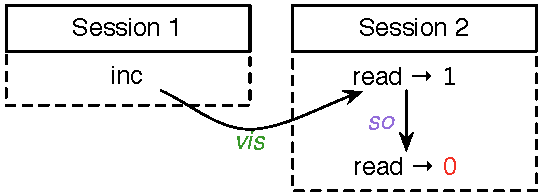
\includegraphics[width=0.55\columnwidth]{Figures/monotonicityViolation}}
%\hfill
\hspace*{0.5in}
\subfigure[Missing
Update]{\label{fig:missingUpdate}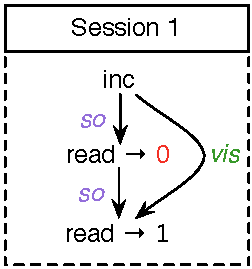
\includegraphics[scale=0.9]{Figures/missingUpdate}}
\hfill
\caption{Anomalies possible under eventual consistency for the counter
read operation.}
\label{fig:counter_anomalies}
\end{figure}

Observe that the counter RDT does not admit a decrement operation.
Therefore, the value of a counter should appear to be monotonically
increasing. Indeed, this property is what makes the RDT useful to
implement, for example, a video view counter on Youtube.
Unfortunately, the monotonicity invariant can be violated in an
eventually consistent execution.

Consider the execution shown in
Figure~\ref{fig:monotonicityViolation}. Session 1 performs an
\rcf{inc} operation on the counter, while Session 2 performs two
\rcf{read} operations. The first \rcf{read} witnesses the effect of
\rcf{inc} from Session 1, hence returns 1. The second \rcf{read},
however, does not witness \rcf{inc}, possibly because it was served by
a replica that has not yet merged the \rcf{inc} effect. It returns 0,
thus violating the monotonicity invariant. 

In order for counter's value to appear monotonically increasing, the
second \rcf{read} should also witness the effect of \rcf{inc}, because
it was witnessed by the preceding \rcf{read}. Because eventually
consistent \rcf{read} operations do not ensure this property,
\rcf{read} operations need to be executed at a stronger consistency
level. The choice of consistency level must guarantee that if
a \rcf{read} witnesses an \rcf{inc} effect, all the subsequent
\rcf{read} operations on the same counter object also witness that
effect. If we let $\sameobjZ$ relate effects over the same
object, we can formalize this requirement using visibility ($\visZ$)
and session order ($\soZ$) relations:
\begin{cmathpar}
\begin{array}{l}
\forall (a : \rcf{inc}), (b,c : \rcf{read}).
\; \vis{a}{b} \conj \so{b}{c} \conj \sameobj{b}{c} \Rightarrow \vis{a}{c} 
\end{array}
\end{cmathpar}
The above formula is in fact a valid specification that can be
associated with counter RDT operations in \name. Note that the
specification captures the guarantees required to enforce the
monotonicity invariant with respect to the abstract model of the store
described in \S~\ref{sec:sysmod}. In particular, the specification
does not refer to the low-level details of any specific data store.
Our observation is that if consistency levels can also be specified in
a similar manner, we can eliminate the need for the application
programmer to understand the low-level nuances of the data store to
enforce the required invariants; understanding their semantics in the
abstract model is enough. In the following sections, we demonstrate
that this is indeed possible. We first introduce our specification
language.

\subsection{Specification Language}

\begin{figure}
\begin{smathpar}
\renewcommand{\arraystretch}{1.2}
\begin{array}{rclcl}
\multicolumn{5}{c}{
  {a,b} \in \mathtt{EffVar} \qquad \qquad
  {\sf Op} \in \mathtt{OperName}
}\\
\cv 		& \in & \mathtt{Spec} 	& \coloneqq & \forall (a : \tau).\cv
        \ALT \forall a.\cv \ALT \pi \\
\tau		& \in	& \mathtt{EffType}	& \coloneqq &  {\sf Op}
        \ALT \tau \vee \tau \\
\pi			&	\in & \mathtt{Prop} & \coloneqq & \true \ALT R(a,b)
        \ALT \pi \vee \pi \\
			  & 		&	 &  \ALT & \pi \wedge \pi \ALT \pi \Rightarrow \pi \\
R				& \in & \mathtt{Relation}	& \coloneqq & \visZ \ALT \soZ
        \ALT \sameobjZ \ALT = \\
				&			&	 &  \ALT & R \cup R \ALT R \cap R \ALT R^+ \\
\end{array}
\end{smathpar}
\caption{Contract language.}
\label{fig:specification-lang}
\end{figure}

The syntax of our specification language is shown in Figure
~\ref{fig:specification-lang}. The language is based on first-order logic
(FOL), and admits prenex universal quantification over typed and
untyped effect variables. We use a special effect variable ($\cureff$)
to denote the effect of the \emph{current operation} - the operation for
which a specification is being written. The type of an effect is
simply the name of the operation (eg: \rcf{inc}) that induced the
effect.  We admit disjunction in types to let an effect variable range
over multiple operation names. The specification $\small \forall (a :
\tau_1 \vee \tau_2).~\psi$ is just syntactic sugar for $\small \forall
a. (\oper{a}{\tau_1} \vee \oper{a}{\tau_2}) \Rightarrow \psi$. An
untyped effect variable ranges over all operation names.

The syntactic class of relations is seeded with primitive $\visZ$,
$\soZ$, and $\sameobjZ$ relations, and also admits derived relations
that are expressible as union, intersection, or transitive closure of
primitive relations. Commonly used derived relations are the
\emph{same object session order} ($\small \sooZ = \soZ ~\cap~
\sameobjZ$), \emph{happens-before order} ($\small \hbZ = (\soZ ~\cup~
\visZ)^+$) and the \emph{same object happens-before order} ($\small
\hboZ = (\sooZ ~\cup~ \visZ)^+$). For example, the same object session
order ($\sooZ$) can be used to succintly represent the specification
of counter RDT's consistency requirement:
\begin{cmathpar}
\begin{array}{l}
\forall (a : \rcf{inc}), (b,c : \rcf{read}).
\; \vis{a}{b} \conj \soo{b}{c} \Rightarrow \vis{a}{c} 
\end{array}
\end{cmathpar}
% Not all syntactically valid \name specifications are well-formed.
% Well-formedness conditions (defined in~\cite{pldi15}) impose certain
% restrictions. For example, a specification can only request visibility
% between effects over same object. Consequently, if a specification is
% an implication, and it contains $\vis{a}{b}$ in its consequent, then
% the antecedent of the implication must imply that $a$ and $b$ are
% effects over the same object (i.e, $\sameobj{a}{b}$). The
% previous specification of counter RDT's requirements is therefore not
% well-formed. Since the consequent contains $\vis{a}{c}$, the
% antecedent of implication should guarantee 

\subsection{Consistency Guarantees}

To help programmers eliminate certain class of anomalies in their
applications, Terry \emph{et al.} equip their data store Bayou~\cite{Bayou}
with four incomparable consistency levels called \emph{session
guarantees}~\cite{Session}. While Terry \emph{et al.} realize efficient
implementations of session guarantees making use of low-level
properties of their store, the semantics of these guarantees can
nonetheless can be captured succintly within \name's abstract model thus:
\begin{smathpar}
\renewcommand{\arraystretch}{1.2}
\begin{array}{rcl}
\R{Read Your Writes (RYW)} & \coloneqq & \forall a,b. ~\soo{a}{b}
\Rightarrow \vis{a}{b} \\
\R{Monotonic Reads (MR)} & \coloneqq & \forall a,b,c. ~\vis{a}{b}
\wedge \soo{b}{c} \Rightarrow \vis{a}{c} \\
\R{Monotonic Writes (MW)} & \coloneqq & \forall a,b,c. ~\soo{a}{b}
\wedge \vis{b}{c} \Rightarrow \vis{a}{c} \\
\R{Writes Follow Reads (WFR)} & \coloneqq & \forall a,b,c,d.
~\vis{a}{b} \wedge \vis{c}{d} \wedge (\sooZ ~\cup =)(b,c) \Rightarrow
\vis{a}{d}
\end{array}
\end{smathpar}
Consider a Monotonic Reads (MR) session guarantee. The semantics of MR
guarantees that if the effect of an operation $a$ is visible to the
effect of $b$, and $b$ precedes $c$ in (same object) session order,
then $a$ will also be made visible to $c$. Recall that this is
precisely the guarantee required by the counter to enforce
monotonicity. In fact, by restricting the bound variable $a$ in MR's
specification to range over \rcf{inc} effects, and bound variables $b$
and $c$ to range over \rcf{read} effects, we can easily conclude that
executing \rcf{read} at an MR consistency level is sufficient to
enforce the monotonicity invariant.

Like MR, the semantics of other session guarantees are categorically
stated by their specifications. Read-Your-Writes (RYW), for example,
guarantees that an operation ($b$) witnesses the effect of every
preceding operation ($a$) in the session. A \rcf{read} operation
executed at RYW consistency level therefore witnesses every previous
\rcf{inc} operation from the same session. This guarantee is necessary
to avoid the anomaly shown in Fig.~\ref{fig:missingUpdate}, where a
\rcf{read} that succeeds an \rcf{inc} fails to witness the effect of
\rcf{inc}, but a later \rcf{read} witnesses the effect. The anomaly
can also be avoided by running \rcf{inc} and \rcf{read} under the
QUORUM consistency level offered by some off-the-shelf key-value
stores, but doing so requires non-trivial reasoning over the semantics
of quorum operations (\emph{e.g.}, strict/sloppy) and conflict
resolution strategies (eg., LWW) to arrive at this conclusion. In
contrast, reasoning with high-level consistency guarantees, such as MR
and RYW, circumvents this complexity.

The precise characterization of guarantees as specifications
facilitates the use of automatic analyses to determine if a
consistency level meets application requirements. For instance,
consider a data store that offers the following three consistency
levels:
\begin{smathpar}
\renewcommand{\arraystretch}{1.2}
\begin{array}{rcl}
\R{Causal Visibility (CV)} & \coloneqq & \forall a,b,c. ~\hbo{a}{b}
\conj \vis{b}{c} \Rightarrow \vis{a}{c} \\
\R{Causal Consistency (CC)} & \coloneqq & \forall a,b,c. ~\hbo{a}{b}
\Rightarrow \vis{a}{b} \\
\R{Strong Consistency (SC)} & \coloneqq & \forall a,b. ~\sameobj{a}{b}
\Rightarrow \vis{a}{b} \vee \vis{b}{c} \\
\end{array}
\end{smathpar}
It is not immediately apparent which among CV, CC and SC meet
the requirements of a counter (CR). Fortunately, we can leverage the power of automated theorem
prover (\emph{e.g.}, Z3)  to prove that the specification of CR is
stronger than CV, but weaker than CC and SC, thus letting us
deduce that counter's requirements can be met both under causal and
strong consistency levels. A theorem prover can also be used to prove that among
CC and SC, CC is weaker. Assuming that weaker guarantees incur
lower cost to enforce availability, it is reasonable to conclude that
counter's \rcf{read} operations should be executed under causal
consistency to enforce  monotonicity. 

The analysis described informally above is formalized as a
\emph{classification scheme}~\cite{pldi15} in \name.  This scheme
completely automates the choice of consistency levels in \name, thus
eliminating the need for programmers to understand the semantics of
different consistency levels. The ease of reasoning with precisely
stated high-level guarantees demonstrates the advantage of exposing
the functionality of the data store via \name, as against the
low-level ad hoc interfaces currently offered by many \ecds.











{
%\small
\bibliographystyle{plainnat} \small \bibliography{all}
}

\end{document}

